This thesis project extends and develops the original Distributed Software Development project, which have been created during the first semester of the 2021 / 2022 academic year. The original project aim was to create a system which could offer photogrammetry services, so the rendering of a tridimensional model from a set of images of the subject, leveraging the container technology to encapsulate the rendering engine. In this section I describe the original architecture of that system and in the next ones I will explain how that architecture has been redesigned, adapted and extended in this thesis project. 

\subsection{System Design}
\label{sse:originalsystemdesign}
  The MapNCloud project was designed as a "three plus one" tiers application:
  \begin{itemize}
    \item a \textbf{presentation layer} or front end, which has been developed as a web site and offers a graphical interface to the system
    \item a \textbf{business layer} or back end, which embodies all the business logic of the application
    \item a \textbf{data layer}, the database which persists the data needed by the application
    \item a \textbf{computation layer}, which is a separated back end module that is tasked with the most computational heavy routines (as the photogrammetry pipelines)
  \end{itemize}
  Another module is present in the application, and it is the ticketing service. It is not considered a whole tier, in fact its only job is to manage the queues of tasks that the backend generates, and let the computational layer components access them in the right order with the right schedule.
  \begin{figure}[H]
    \centering
    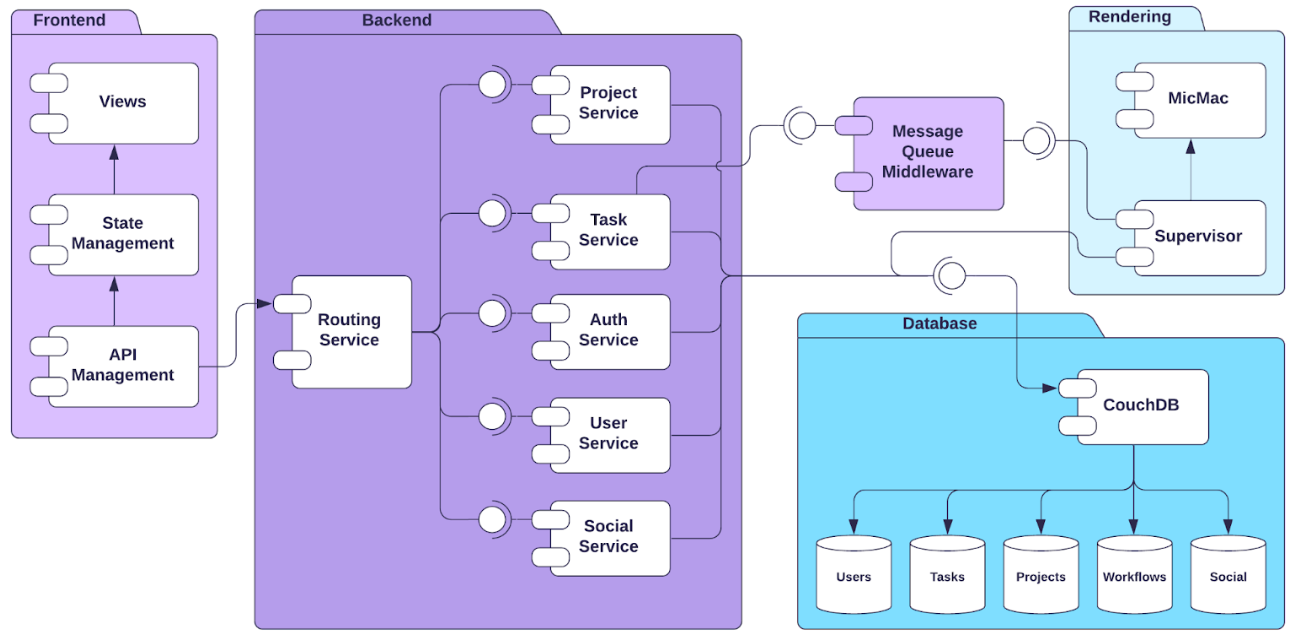
\includegraphics[width = \textwidth]{../Images/MNCOriginal.png}
    \caption{Original MapNCloud component diagram, with internal modules detailed.}
  \end{figure}

  \subsubsection{Front End}
  \label{ssse:originalfrontend}
    The presentation layer of the application was developed as a web application; this exposes a graphical user interface for the services offered by the system. It is a JavaScript application (developed with the VueJS framework) which interacts with the backend via HTTP calls; this allows it to be considered, by the cloud provider, a static web application, which is easy to deploy and has a low resources demand.\\
    The front end architecture follows the Model View ViewModel pattern, which separates the actual GUI elements from the logic of the user experience in View and ViewModel respectively, and lets the ViewModel reflect the changes on the Model; this is a common pattern to adopt as it provides a clear organization of functionalities and responsibilities among the internal software submodules.\\
    The front end module is the one that is the least affected by this thesis work; it is only extended to include an admininitration section.

  \subsubsection{Back End}
  \label{ssse:originalbackend}

  \subsubsection{Computation Later}
  \label{ssse:originalcomputationlayer}
